%%% Template originaly created by Karol Kozioł (mail@karol-koziol.net) and modified for ShareLaTeX use

\documentclass[a4paper,11pt]{article}

\usepackage[T1]{fontenc}
\usepackage[utf8]{inputenc}
\usepackage[utf8]{vietnam}
\usepackage{graphicx}
\usepackage{xcolor}
\renewcommand\familydefault{\sfdefault}
\usepackage{tgheros}
\usepackage[defaultmono]{droidmono}
\usepackage{amsmath,amssymb,amsthm,textcomp}
\usepackage{enumerate}
\usepackage{multicol}
\usepackage{tikz}
\usepackage{geometry}
\geometry{left=25mm,right=25mm,%
bindingoffset=0mm, top=20mm,bottom=20mm}
\linespread{1.3}
\newcommand{\linia}{\rule{\linewidth}{0.5pt}}
% custom theorems if needed
\newtheoremstyle{mytheor}
    {1ex}{1ex}{\normalfont}{0pt}{\scshape}{.}{1ex}
    {{\thmname{#1 }}{\thmnumber{#2}}{\thmnote{ (#3)}}}
\theoremstyle{mytheor}
\newtheorem{defi}{Definition}
% my own titles
\makeatletter
\renewcommand{\maketitle}{
\begin{center}
\vspace{2ex}
{\huge \textsc{\@title}}
\vspace{1ex}
\\
\linia\\
\@author \hfill \@date
\vspace{4ex}
\end{center}
}
\makeatother
%%%

% custom footers and headers
\usepackage{fancyhdr}
\pagestyle{fancy}
\lhead{}
\chead{}
\rhead{}
\lfoot{}
\cfoot{}
\rfoot{Page \thepage}
\renewcommand{\headrulewidth}{0pt}
\renewcommand{\footrulewidth}{0pt}
%

% code listing settings
\usepackage{listings}
\lstset{
    language=Python,
    basicstyle=\ttfamily\small,
    aboveskip={1.0\baselineskip},
    belowskip={1.0\baselineskip},
    columns=fixed,
    extendedchars=true,
    breaklines=true,
    tabsize=4,
    prebreak=\raisebox{0ex}[0ex][0ex]{\ensuremath{\hookleftarrow}},
    frame=lines,
    showtabs=false,
    showspaces=false,
    showstringspaces=false,
    keywordstyle=\color[rgb]{0.627,0.126,0.941},
    commentstyle=\color[rgb]{0.133,0.545,0.133},
    stringstyle=\color[rgb]{01,0,0},
    numbers=left,
    numberstyle=\small,
    stepnumber=1,
    numbersep=10pt,
    captionpos=t,
    escapeinside={\%*}{*)}
}
\usepackage{hyperref}
\hypersetup{
    colorlinks=true,
    linkcolor=blue,
    filecolor=magenta,      
    urlcolor=cyan,
}
\usepackage{amsmath}
\makeatletter
\renewcommand*\env@matrix[1][*\c@MaxMatrixCols c]{%
  \hskip -\arraycolsep
  \let\@ifnextchar\new@ifnextchar
  \array{#1}}
\makeatother
%%%----------%%%----------%%%----------%%%----------%%%

\begin{document}

\title{Lecture 2 Assignment}

\author{Nguyen Quang Huy}

\date{31/03/2020}

\maketitle

\section*{P2.1}

Bằng cách viết phép biến đổi affin $T_bx = Ax+b$ với $A \in R^{n*n},x,b\in R^n$ dưới dạng một biến đổi tuyến tính $T_bx = \overline{A}*\overline{x}$ với $\overline{A}= \begin{bmatrix}[c|c] A &  b \\0 ... 0  & 1\\ \end{bmatrix}$ và $\overline{x} = \begin{bmatrix}x\\1\end{bmatrix}$, ta có thể kết hợp chuỗi biến đổi gồm nhiều phép biến đổi affin thành 1 ma trận duy nhất bằng phép nhân các ma trận tương ứng.\\
\\
VD: kết hợp rời hình theo vector $\{5;10\}$, phóng hình với tỷ lệ $\{1,2;1,5\}$ và xoay hình $30^o$:
\begin{align}
    \nonumber \overline{R}*(\overline{S}*(\overline{T}*\overline{x}))  &= Rotate(\frac{\pi}{6}) * Scale(1.2,1.5) * Translate(5,10) * x \\
    \nonumber &= \begin{bmatrix} cos\frac{\pi}{6} & sin\frac{\pi}{6} & 0 \\ -sin\frac{\pi}{6} & cos\frac{\pi}{6} & 0 \\ 0 & 0 & 1\end{bmatrix} * 
        \begin{bmatrix} 1.2 & 0 & 0 \\ 0 & 1.5 & 0 \\ 0 & 0& 1\end{bmatrix} * 
        \begin{bmatrix} 1 & 0 & 5 \\ 0 & 1 & 10 \\ 0 & 0 & 1\end{bmatrix} *
        \begin{bmatrix} x_1 \\ x_2 \\ 1 \end{bmatrix}
        \\
    \nonumber &= \begin{bmatrix} 1.03923048 & 0.75 & 12.69615242 \\ -0.6 & 1.29903811 & 9.99038106 \\ 0 & 0& 1 \end{bmatrix} * \begin{bmatrix} x_1 \\ x_2 \\ 1 \end{bmatrix}
\end{align}
\\
\\
Kết quả phép biến đổi $\overline{A}$: < \href{https://drive.google.com/open?id=1cn1MvcO2GaH6VP82nk3vjckOZAmmLQwO}{P2.1.gif} >

\begin{multicols}{2}
\centering
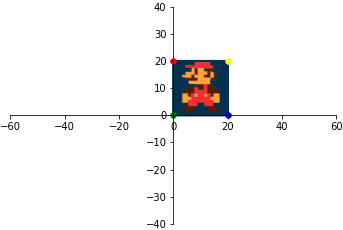
\includegraphics[width=0.5\textwidth]{P2_1_01.png}
\\Input
\columnbreak
\\
\centering
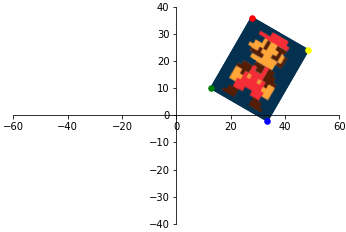
\includegraphics[width=0.5\textwidth]{P2_1_02.png}
\\Output
\end{multicols}

Nhận xét: việc đưa thêm 1 hàng ở dưới ma trận A giúp ma trận $\overline{A}$ trở thành ma trận vuông n*n, giúp có thể kết hợp chuỗi biến đổi với nhau bằng cách nhân ma trận theo thứ tự tương ứng.Ngoài ra dòng được thêm vào không thay đổi sau phép nhân ma trận. 


\section*{P2.2}
4 không gian con cơ bản gồm không gian cột và không gian hạch của ma trận $A$ và $A^T$

\subsection*{Tính chất 1}
Với ma trận $A_{n*m}$, không gian cột và không gian hàng có số chiều bằng nhau, không gian hạch $N(A)$ có số chiều bằng n-r, không gian hạch $N(A^T)$ có số chiều m-r
$$r = rank(A) = rank(A^T)$$
$$Nullity(A) = n-r $$
$$Nullity(A^T) = m-r$$

\subsection*{Tính chất 2}
Không gian cột và không gian hạch $N(A^T)$ là trực giao.\\
Không gian hàng và không gian hạch $N(A)$ là trực giao. 

\subsection*{Tính chất 3}
Phương trình:
    $$A*x = \lambda*x$$
trong đó:

x là vector riêng của A

$\lambda$ là giá trị riêng tương ứng với vector riêng của A

Vector riêng của một biến đổi tuyến tính là vector khác vector $\bar{0}$, có tính chất vẫn giữ nguyên chiều khi đưa vào phép biến đổi. Giá trị riêng thể hiện sự thay đổi của vector riêng khi đưa vào phép biến đổi.\\

\begin{multicols}{2}
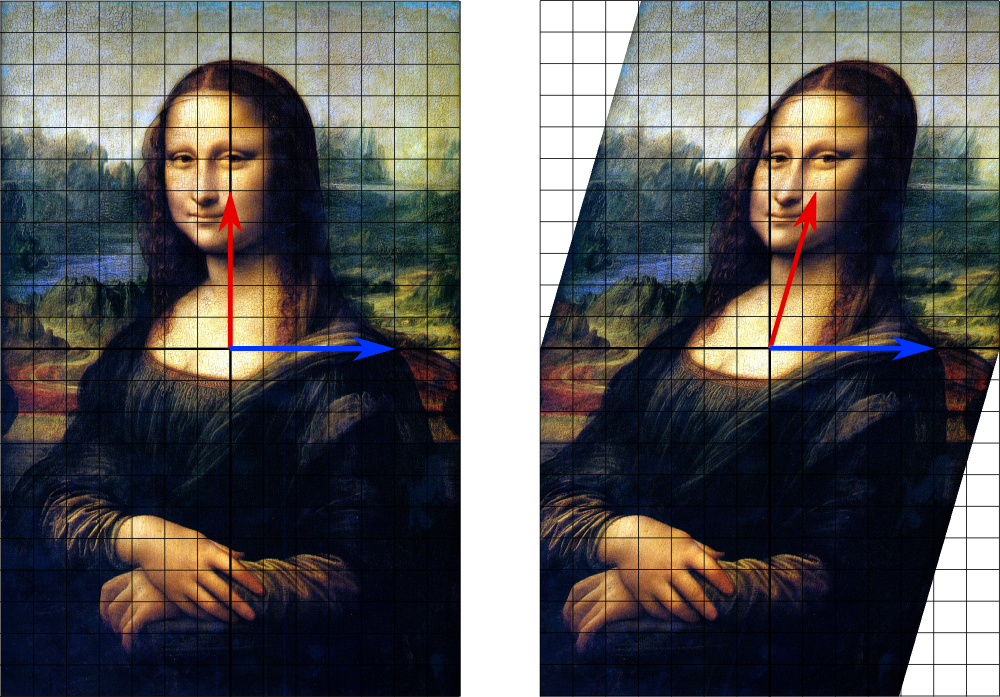
\includegraphics[width=0.45\textwidth]{P2_2_01.png}
\columnbreak
\\
Xét T(x) = Ax\\
Ở đây ta thấy vector màu xanh vẫn giữ nguyên hướng nên nó là vector riêng của A, do chiều dài vector giữ nguyên nên giá trị riêng tương ứng của nó là 1. Vector đỏ không phải là vector riêng.
\end{multicols}

v = $\{v_1,v_2,...v_n\}$ là các vector riêng của $A$, với các giá trị riêng $\sigma^2>=0$
u = $\{u_1,u_2,...u_n\}$ là các vector riêng của $A^T$

\section*{P2.3}
Chứng minh phép nhân ma trận $\tau: R^{n*p} \xrightarrow{} R^{m*p}$ với $\tau C=D, \tau = B_{m*n}$ là một ánh xạ tuyến tính
\subsection*{Chứng minh T(au+bv) = aTu+bTv:}
Với $X_1,X_2 \in R_{n*p}$, ta có:
\begin{align}
    \nonumber\tau(a*X_1+b*X_2) &= B*(a*X_1+b*X_2)\\
    \nonumber&= B*a*X_1 + B*b*X_2\\
    \nonumber&= a*B*X_1 + b*B*X_2\\
    \nonumber&= a*\tau(X_1) + b*\tau(X_2)
\end{align}
\subsubsection*{Chứng minh đầu vào và đầu ra có tính kết hợp và tổng hợp giống nhau:}
Với $X_1,X_2 \in R_{n*p}, Y_1,Y_2 \in R_{m*p}, \tau(X_1) = Y_1, \tau(X_2) = Y_2$, ta có:
\begin{itemize}
    \item $X_1+X_2$ tỷ lệ với $Y_1+Y_2$
    \item $a*X_1$ tỷ lệ với $a*Y_1$
\end{itemize}
Vậy phép nhân ma trận $\tau: R^{n*p} \xrightarrow{} R^{m*p}$ là một ánh xạ tuyến tính.

Với A = $\begin{bmatrix}1&2\\0&1\end{bmatrix}$, ta có:
$$
    A*B = \begin{bmatrix}1&2\\0&1\end{bmatrix} * \begin{bmatrix}x_{1 1}&x_{1 2}\\x_{2 1}&x_{2 2}\end{bmatrix} = \begin{bmatrix}x_{1 1} + 2x_{2 1}&x_{1 2} + 2x_{2 2}\\x_{2 1}&x_{2 2}\end{bmatrix}
$$
ma trận biểu diễn biến đổi tuyến tính trong standard bases:

Với $\bar{A} = \begin{bmatrix}1&2&0&0\\0&1&0&0\\0&0&1&2\\0&0&0&1\end{bmatrix}$, ta có:
$$
    \bar{A}*\bar{B} = \begin{bmatrix}1&2&0&0\\0&1&0&0\\0&0&1&2\\0&0&0&1\end{bmatrix} * \begin{bmatrix}x_{1 1}\\x_{2 1}\\x_{1 2}\\x_{2 2}\end{bmatrix} = \begin{bmatrix}x_{1 1} + 2x_{2 1}\\x_{2 1}\\x_{1 2} + 2x_{2 2}\\x_{2 2}\end{bmatrix}
$$

\section*{P2.4}
\subsection*{Chứng minh ker(f) là không gian con của $R^5$ với f: $R^5\xrightarrow{}R^5$}
Ker(f) là tập con của không gian $R^5$, do với $x_1,x_2 \in ker(f)$, ta có $(x_1+x_2) \in ker(f)$, $a*x_1 \in ker(f) \forall a \in R$ nên ker(f) là không gian con của $R^5$.
\subsection*{Chứng minh f là hàm tuyến tính}
Với $f(x_1,x_2,...x_5) = (x_1,x_2,x_3,x_4,0)$, f là hàm tuyến tính vì f có thể viết được dưới dạng y = Ax+b.\\ Trong đó:
A = $\begin{bmatrix}1&0&0&0&0\\ 0&1&0&0&0 \\ 0&0&1&0&0 \\ 0&0&0&1&0 \\ 0&0&0&0&0 \end{bmatrix}$ và b = 0, 
kef(f) = span\{(0,0,0,0,1)\}, dim(ker(f)) = 1.
\section*{C2.1}
\href{https://colab.research.google.com/drive/1tHw-s6tutmhnt6YglAT1ct_C_fjuwaMu}{Code link here}
\\
\href{https://drive.google.com/open?id=1CMKWzSm0z0JqbRqxY4HaTwfDtyS0LSvh}{Gif link here}
\section*{C2.2}
\section*{C2.3}
\section*{C2.4}
Bài này em tham khảo code của Machine Learning cơ bản :/ Nhưng cảm thấy ko phát triểnđược nhiều lắm.\\
\href{https://colab.research.google.com/drive/1WbQtkARnAL2FdrglXXfmRoXAN40OF712}{Code link here}
\section*{C2.5}

\section*{E2.1}
Giả thiết sai vì một biến đổi tuyến tính không phải map one to one\\
Sửa lại:
$$T(\sum_{i=1}^n a_i v_i) = T(v) \xleftarrow{} \sum_{i=1}^n a_i v_i = v$$
\section*{E2.2}
Giả sử tồn tại T : V $\xrightarrow{}$ W = Ax với $A \in R^{n*n}$ thỏa mãn:
    $$\forall j \in 1,...,n,T(v_j) = w_j$$
Ta định nghĩa 2 ma trận:
$$
    X  =  [v_1,v_2,...,v_n]
$$
$$
    W  =  [w_1,w_2,...,w_n]
$$
Do X là hệ cơ sở của không gian V nên X độc lập tuyến tính, do đó dim(X) $\neq$ 0 $\xrightarrow{} $ X khả nghịch (1) 
Ta có
\begin{align}
    \nonumber A*X &= W\\
    \nonumber\xrightarrow{}A*X*X^{-1} &= W*X^{-1}\\
    \nonumber\xrightarrow{}A &= W*X^{-1}
\end{align}
Vậy tồn tại duy nhất 1 ma trận A thỏa mãn
\section*{E2.3}
Nhân ma trận thể hiện việc giải nhiều phương trình/ hệ phương trình tương đồng nhau một cách đồng thời, giúp thể hiện việc giải hệ phương trình nhìn trực quan hơn.
\section*{E2.4}
Với ma trận A là $\begin{bmatrix}
        a_{1 1} & a_{1 2} & \dots & a_{1 m}\\
        a_{2 1} & a_{2 2} & \dots & a_{2 m}\\
        \vdots & \vdots & \ddots & \vdots \\
        a_{n 1} & a_{n 2} & \dots & a_{n m}
        \end{bmatrix} 
        = \begin{bmatrix}
        a_1 \\ a_2 \\ \vdots \\ a_n
        \end{bmatrix}
        $ 
\\
\\
Ta có hệ cơ sở V = $[v_1,v_2,...,v_t]$ là hệ cơ sở của không gian hàng của A, suy ra mọi vector $v_1,v_2,...,v_t$ đều viết được dưới dạng tổ hợp tuyến tính của các vector$a_1,a_2,...,a_n$ .\\
Theo định nghĩa, không gian hạch của ma trận A là $\{x | Ax = \bar{0}\}$, hay $\{x|a_i*x = 0 \forall i \in [1,n]\}$, hay $\{x|v_i*x = 0 \forall i \in [1,t]\}$\\
Suy ra mọi vector x thuộc không gian hạch đều trực giao với mọi vector $v_i$ hay mọi vector x thuộc không gian hạch đều trực giao với mọi vector trong span(v) (không gian hàng của A).
\section*{E2.5}
B1: Giải ma trận $Ax=\bar{0}$ theo khai triển Gauss-Johndan, thu được ma trận $\bar{A}$ gồm r hàng bằng 0 và n-r hàng khác vector 0.\\
B2: Không gian hàng của ma trận A = span(n-r hàng khác 0).\\
B3: Không gian hạch của ma trận A là không gian nghiệm của phương trình $\bar{A}x=\bar{0}$.
\section*{E2.6}
Với số cặp thỏ con $A_i$ và số cặp thỏ trưởng thành $B_i$ thì số cặp thỏ trưởng thành năm tiếp theo là $B_{i+1}= A_i*(1-p_a)+B_i*(1-p_c)$ và số cặp thỏ con năm tiếp theo $A_{i+1} = B_i*(1-p_c)*p_b$.\\
Trong đó:
\begin{itemize}
\item Tỷ lệ sinh sản $p_b$ : số cặp thỏ con trung bình mà 1 cặp thỏ trưởng thành sinh sản trong 1 năm.
\item Tỷ lệ tử vong thỏ con $p_c$ : tỷ lệ tử vong của 1 cặp thỏ con trong 1 năm.
\item Tỷ lệ tử vong thỏ trưởng thành $p_a$ : tỷ lệ tử vong của 1 cặp thỏ trưởng thành trong 1 năm.
\end{itemize}
Viết lại hệ dưới cách biểu diễn bằng ma trận:\\
$$
    \begin{bmatrix}0&(1-p_c)*p_b\\ 1-p_a & 1-p_c \end{bmatrix} * \begin{bmatrix}A_i\\B_i\end{bmatrix} = \begin{bmatrix}A_{i+1}\\B_{i+1}\end{bmatrix}
$$
Tổng quát sau t năm:
$$
    \begin{bmatrix}0&(1-p_c)*p_b\\ 1-p_a & 1-p_c \end{bmatrix}^t * \begin{bmatrix}A_i\\B_i\end{bmatrix} = \begin{bmatrix}A_{i+t}\\B_{i+t}\end{bmatrix}
$$
Để tính tổng số cặp thỏ sau t năm, ta cộng tổng số cặp thỏ trưởng thành và số cặp thỏ con sau t năm:
$$
    \begin{bmatrix}1 & 1\end{bmatrix}*
    \begin{bmatrix}0&(1-p_c)*p_b\\ 1-p_a & 1-p_c \end{bmatrix}^t * \begin{bmatrix}A_i\\B_i\end{bmatrix} = A_{i+t}+B_{i+t}
$$
Vậy ta xây dựng được phương trình f() = ax với a = $\begin{bmatrix}1 & 1\end{bmatrix}* \begin{bmatrix}0&(1-p_c)*p_b\\ 1-p_a & 1-p_c \end{bmatrix}^t$\\
Xây dựng phương trình f() = ax với $p_a \sim U(a_l,a_u),p_b \sim U(b_l,b_u),p_c \sim U(c_l,c_u) $:
\begin{itemize}
    \item $f_u$ với a =  $\begin{bmatrix}1 & 1\end{bmatrix}* \begin{bmatrix}0&(1-c_l)*b_u\\ 1-a_l & 1-c_l \end{bmatrix}^t$
    \item $f_l$ = ax với a =  $\begin{bmatrix}1 & 1\end{bmatrix}* \begin{bmatrix}0&(1-c_u)*b_l\\ 1-a_u & 1-c_u \end{bmatrix}^t$
\end{itemize}
\end{document}
